\documentclass[11pt]{article}

    \usepackage[breakable]{tcolorbox}
    \usepackage{parskip} % Stop auto-indenting (to mimic markdown behaviour)
    
    \usepackage{iftex}
    \ifPDFTeX
    	\usepackage[T1]{fontenc}
    	\usepackage{mathpazo}
    \else
    	\usepackage{fontspec}
    \fi

    % Basic figure setup, for now with no caption control since it's done
    % automatically by Pandoc (which extracts ![](path) syntax from Markdown).
    \usepackage{graphicx}
    % Maintain compatibility with old templates. Remove in nbconvert 6.0
    \let\Oldincludegraphics\includegraphics
    % Ensure that by default, figures have no caption (until we provide a
    % proper Figure object with a Caption API and a way to capture that
    % in the conversion process - todo).
    \usepackage{caption}
    \DeclareCaptionFormat{nocaption}{}
    \captionsetup{format=nocaption,aboveskip=0pt,belowskip=0pt}

    \usepackage[Export]{adjustbox} % Used to constrain images to a maximum size
    \adjustboxset{max size={0.9\linewidth}{0.9\paperheight}}
    \usepackage{float}
    \floatplacement{figure}{H} % forces figures to be placed at the correct location
    \usepackage{xcolor} % Allow colors to be defined
    \usepackage{enumerate} % Needed for markdown enumerations to work
    \usepackage{geometry} % Used to adjust the document margins
    \usepackage{amsmath} % Equations
    \usepackage{amssymb} % Equations
    \usepackage{textcomp} % defines textquotesingle
    % Hack from http://tex.stackexchange.com/a/47451/13684:
    \AtBeginDocument{%
        \def\PYZsq{\textquotesingle}% Upright quotes in Pygmentized code
    }
    \usepackage{upquote} % Upright quotes for verbatim code
    \usepackage{eurosym} % defines \euro
    \usepackage[mathletters]{ucs} % Extended unicode (utf-8) support
    \usepackage{fancyvrb} % verbatim replacement that allows latex
    \usepackage{grffile} % extends the file name processing of package graphics 
                         % to support a larger range
    \makeatletter % fix for grffile with XeLaTeX
    \def\Gread@@xetex#1{%
      \IfFileExists{"\Gin@base".bb}%
      {\Gread@eps{\Gin@base.bb}}%
      {\Gread@@xetex@aux#1}%
    }
    \makeatother

    % The hyperref package gives us a pdf with properly built
    % internal navigation ('pdf bookmarks' for the table of contents,
    % internal cross-reference links, web links for URLs, etc.)
    \usepackage{hyperref}
    % The default LaTeX title has an obnoxious amount of whitespace. By default,
    % titling removes some of it. It also provides customization options.
    \usepackage{titling}
    \usepackage{longtable} % longtable support required by pandoc >1.10
    \usepackage{booktabs}  % table support for pandoc > 1.12.2
    \usepackage[inline]{enumitem} % IRkernel/repr support (it uses the enumerate* environment)
    \usepackage[normalem]{ulem} % ulem is needed to support strikethroughs (\sout)
                                % normalem makes italics be italics, not underlines
    \usepackage{mathrsfs}
    

    
    % Colors for the hyperref package
    \definecolor{urlcolor}{rgb}{0,.145,.698}
    \definecolor{linkcolor}{rgb}{.71,0.21,0.01}
    \definecolor{citecolor}{rgb}{.12,.54,.11}

    % ANSI colors
    \definecolor{ansi-black}{HTML}{3E424D}
    \definecolor{ansi-black-intense}{HTML}{282C36}
    \definecolor{ansi-red}{HTML}{E75C58}
    \definecolor{ansi-red-intense}{HTML}{B22B31}
    \definecolor{ansi-green}{HTML}{00A250}
    \definecolor{ansi-green-intense}{HTML}{007427}
    \definecolor{ansi-yellow}{HTML}{DDB62B}
    \definecolor{ansi-yellow-intense}{HTML}{B27D12}
    \definecolor{ansi-blue}{HTML}{208FFB}
    \definecolor{ansi-blue-intense}{HTML}{0065CA}
    \definecolor{ansi-magenta}{HTML}{D160C4}
    \definecolor{ansi-magenta-intense}{HTML}{A03196}
    \definecolor{ansi-cyan}{HTML}{60C6C8}
    \definecolor{ansi-cyan-intense}{HTML}{258F8F}
    \definecolor{ansi-white}{HTML}{C5C1B4}
    \definecolor{ansi-white-intense}{HTML}{A1A6B2}
    \definecolor{ansi-default-inverse-fg}{HTML}{FFFFFF}
    \definecolor{ansi-default-inverse-bg}{HTML}{000000}

    % commands and environments needed by pandoc snippets
    % extracted from the output of `pandoc -s`
    \providecommand{\tightlist}{%
      \setlength{\itemsep}{0pt}\setlength{\parskip}{0pt}}
    \DefineVerbatimEnvironment{Highlighting}{Verbatim}{commandchars=\\\{\}}
    % Add ',fontsize=\small' for more characters per line
    \newenvironment{Shaded}{}{}
    \newcommand{\KeywordTok}[1]{\textcolor[rgb]{0.00,0.44,0.13}{\textbf{{#1}}}}
    \newcommand{\DataTypeTok}[1]{\textcolor[rgb]{0.56,0.13,0.00}{{#1}}}
    \newcommand{\DecValTok}[1]{\textcolor[rgb]{0.25,0.63,0.44}{{#1}}}
    \newcommand{\BaseNTok}[1]{\textcolor[rgb]{0.25,0.63,0.44}{{#1}}}
    \newcommand{\FloatTok}[1]{\textcolor[rgb]{0.25,0.63,0.44}{{#1}}}
    \newcommand{\CharTok}[1]{\textcolor[rgb]{0.25,0.44,0.63}{{#1}}}
    \newcommand{\StringTok}[1]{\textcolor[rgb]{0.25,0.44,0.63}{{#1}}}
    \newcommand{\CommentTok}[1]{\textcolor[rgb]{0.38,0.63,0.69}{\textit{{#1}}}}
    \newcommand{\OtherTok}[1]{\textcolor[rgb]{0.00,0.44,0.13}{{#1}}}
    \newcommand{\AlertTok}[1]{\textcolor[rgb]{1.00,0.00,0.00}{\textbf{{#1}}}}
    \newcommand{\FunctionTok}[1]{\textcolor[rgb]{0.02,0.16,0.49}{{#1}}}
    \newcommand{\RegionMarkerTok}[1]{{#1}}
    \newcommand{\ErrorTok}[1]{\textcolor[rgb]{1.00,0.00,0.00}{\textbf{{#1}}}}
    \newcommand{\NormalTok}[1]{{#1}}
    
    % Additional commands for more recent versions of Pandoc
    \newcommand{\ConstantTok}[1]{\textcolor[rgb]{0.53,0.00,0.00}{{#1}}}
    \newcommand{\SpecialCharTok}[1]{\textcolor[rgb]{0.25,0.44,0.63}{{#1}}}
    \newcommand{\VerbatimStringTok}[1]{\textcolor[rgb]{0.25,0.44,0.63}{{#1}}}
    \newcommand{\SpecialStringTok}[1]{\textcolor[rgb]{0.73,0.40,0.53}{{#1}}}
    \newcommand{\ImportTok}[1]{{#1}}
    \newcommand{\DocumentationTok}[1]{\textcolor[rgb]{0.73,0.13,0.13}{\textit{{#1}}}}
    \newcommand{\AnnotationTok}[1]{\textcolor[rgb]{0.38,0.63,0.69}{\textbf{\textit{{#1}}}}}
    \newcommand{\CommentVarTok}[1]{\textcolor[rgb]{0.38,0.63,0.69}{\textbf{\textit{{#1}}}}}
    \newcommand{\VariableTok}[1]{\textcolor[rgb]{0.10,0.09,0.49}{{#1}}}
    \newcommand{\ControlFlowTok}[1]{\textcolor[rgb]{0.00,0.44,0.13}{\textbf{{#1}}}}
    \newcommand{\OperatorTok}[1]{\textcolor[rgb]{0.40,0.40,0.40}{{#1}}}
    \newcommand{\BuiltInTok}[1]{{#1}}
    \newcommand{\ExtensionTok}[1]{{#1}}
    \newcommand{\PreprocessorTok}[1]{\textcolor[rgb]{0.74,0.48,0.00}{{#1}}}
    \newcommand{\AttributeTok}[1]{\textcolor[rgb]{0.49,0.56,0.16}{{#1}}}
    \newcommand{\InformationTok}[1]{\textcolor[rgb]{0.38,0.63,0.69}{\textbf{\textit{{#1}}}}}
    \newcommand{\WarningTok}[1]{\textcolor[rgb]{0.38,0.63,0.69}{\textbf{\textit{{#1}}}}}
    
    
    % Define a nice break command that doesn't care if a line doesn't already
    % exist.
    \def\br{\hspace*{\fill} \\* }
    % Math Jax compatibility definitions
    \def\gt{>}
    \def\lt{<}
    \let\Oldtex\TeX
    \let\Oldlatex\LaTeX
    \renewcommand{\TeX}{\textrm{\Oldtex}}
    \renewcommand{\LaTeX}{\textrm{\Oldlatex}}
    % Document parameters
    % Document title
    \title{proj\_opti\_chesneaux\_plessix}
    
    
    
    
    
% Pygments definitions
\makeatletter
\def\PY@reset{\let\PY@it=\relax \let\PY@bf=\relax%
    \let\PY@ul=\relax \let\PY@tc=\relax%
    \let\PY@bc=\relax \let\PY@ff=\relax}
\def\PY@tok#1{\csname PY@tok@#1\endcsname}
\def\PY@toks#1+{\ifx\relax#1\empty\else%
    \PY@tok{#1}\expandafter\PY@toks\fi}
\def\PY@do#1{\PY@bc{\PY@tc{\PY@ul{%
    \PY@it{\PY@bf{\PY@ff{#1}}}}}}}
\def\PY#1#2{\PY@reset\PY@toks#1+\relax+\PY@do{#2}}

\expandafter\def\csname PY@tok@w\endcsname{\def\PY@tc##1{\textcolor[rgb]{0.73,0.73,0.73}{##1}}}
\expandafter\def\csname PY@tok@c\endcsname{\let\PY@it=\textit\def\PY@tc##1{\textcolor[rgb]{0.25,0.50,0.50}{##1}}}
\expandafter\def\csname PY@tok@cp\endcsname{\def\PY@tc##1{\textcolor[rgb]{0.74,0.48,0.00}{##1}}}
\expandafter\def\csname PY@tok@k\endcsname{\let\PY@bf=\textbf\def\PY@tc##1{\textcolor[rgb]{0.00,0.50,0.00}{##1}}}
\expandafter\def\csname PY@tok@kp\endcsname{\def\PY@tc##1{\textcolor[rgb]{0.00,0.50,0.00}{##1}}}
\expandafter\def\csname PY@tok@kt\endcsname{\def\PY@tc##1{\textcolor[rgb]{0.69,0.00,0.25}{##1}}}
\expandafter\def\csname PY@tok@o\endcsname{\def\PY@tc##1{\textcolor[rgb]{0.40,0.40,0.40}{##1}}}
\expandafter\def\csname PY@tok@ow\endcsname{\let\PY@bf=\textbf\def\PY@tc##1{\textcolor[rgb]{0.67,0.13,1.00}{##1}}}
\expandafter\def\csname PY@tok@nb\endcsname{\def\PY@tc##1{\textcolor[rgb]{0.00,0.50,0.00}{##1}}}
\expandafter\def\csname PY@tok@nf\endcsname{\def\PY@tc##1{\textcolor[rgb]{0.00,0.00,1.00}{##1}}}
\expandafter\def\csname PY@tok@nc\endcsname{\let\PY@bf=\textbf\def\PY@tc##1{\textcolor[rgb]{0.00,0.00,1.00}{##1}}}
\expandafter\def\csname PY@tok@nn\endcsname{\let\PY@bf=\textbf\def\PY@tc##1{\textcolor[rgb]{0.00,0.00,1.00}{##1}}}
\expandafter\def\csname PY@tok@ne\endcsname{\let\PY@bf=\textbf\def\PY@tc##1{\textcolor[rgb]{0.82,0.25,0.23}{##1}}}
\expandafter\def\csname PY@tok@nv\endcsname{\def\PY@tc##1{\textcolor[rgb]{0.10,0.09,0.49}{##1}}}
\expandafter\def\csname PY@tok@no\endcsname{\def\PY@tc##1{\textcolor[rgb]{0.53,0.00,0.00}{##1}}}
\expandafter\def\csname PY@tok@nl\endcsname{\def\PY@tc##1{\textcolor[rgb]{0.63,0.63,0.00}{##1}}}
\expandafter\def\csname PY@tok@ni\endcsname{\let\PY@bf=\textbf\def\PY@tc##1{\textcolor[rgb]{0.60,0.60,0.60}{##1}}}
\expandafter\def\csname PY@tok@na\endcsname{\def\PY@tc##1{\textcolor[rgb]{0.49,0.56,0.16}{##1}}}
\expandafter\def\csname PY@tok@nt\endcsname{\let\PY@bf=\textbf\def\PY@tc##1{\textcolor[rgb]{0.00,0.50,0.00}{##1}}}
\expandafter\def\csname PY@tok@nd\endcsname{\def\PY@tc##1{\textcolor[rgb]{0.67,0.13,1.00}{##1}}}
\expandafter\def\csname PY@tok@s\endcsname{\def\PY@tc##1{\textcolor[rgb]{0.73,0.13,0.13}{##1}}}
\expandafter\def\csname PY@tok@sd\endcsname{\let\PY@it=\textit\def\PY@tc##1{\textcolor[rgb]{0.73,0.13,0.13}{##1}}}
\expandafter\def\csname PY@tok@si\endcsname{\let\PY@bf=\textbf\def\PY@tc##1{\textcolor[rgb]{0.73,0.40,0.53}{##1}}}
\expandafter\def\csname PY@tok@se\endcsname{\let\PY@bf=\textbf\def\PY@tc##1{\textcolor[rgb]{0.73,0.40,0.13}{##1}}}
\expandafter\def\csname PY@tok@sr\endcsname{\def\PY@tc##1{\textcolor[rgb]{0.73,0.40,0.53}{##1}}}
\expandafter\def\csname PY@tok@ss\endcsname{\def\PY@tc##1{\textcolor[rgb]{0.10,0.09,0.49}{##1}}}
\expandafter\def\csname PY@tok@sx\endcsname{\def\PY@tc##1{\textcolor[rgb]{0.00,0.50,0.00}{##1}}}
\expandafter\def\csname PY@tok@m\endcsname{\def\PY@tc##1{\textcolor[rgb]{0.40,0.40,0.40}{##1}}}
\expandafter\def\csname PY@tok@gh\endcsname{\let\PY@bf=\textbf\def\PY@tc##1{\textcolor[rgb]{0.00,0.00,0.50}{##1}}}
\expandafter\def\csname PY@tok@gu\endcsname{\let\PY@bf=\textbf\def\PY@tc##1{\textcolor[rgb]{0.50,0.00,0.50}{##1}}}
\expandafter\def\csname PY@tok@gd\endcsname{\def\PY@tc##1{\textcolor[rgb]{0.63,0.00,0.00}{##1}}}
\expandafter\def\csname PY@tok@gi\endcsname{\def\PY@tc##1{\textcolor[rgb]{0.00,0.63,0.00}{##1}}}
\expandafter\def\csname PY@tok@gr\endcsname{\def\PY@tc##1{\textcolor[rgb]{1.00,0.00,0.00}{##1}}}
\expandafter\def\csname PY@tok@ge\endcsname{\let\PY@it=\textit}
\expandafter\def\csname PY@tok@gs\endcsname{\let\PY@bf=\textbf}
\expandafter\def\csname PY@tok@gp\endcsname{\let\PY@bf=\textbf\def\PY@tc##1{\textcolor[rgb]{0.00,0.00,0.50}{##1}}}
\expandafter\def\csname PY@tok@go\endcsname{\def\PY@tc##1{\textcolor[rgb]{0.53,0.53,0.53}{##1}}}
\expandafter\def\csname PY@tok@gt\endcsname{\def\PY@tc##1{\textcolor[rgb]{0.00,0.27,0.87}{##1}}}
\expandafter\def\csname PY@tok@err\endcsname{\def\PY@bc##1{\setlength{\fboxsep}{0pt}\fcolorbox[rgb]{1.00,0.00,0.00}{1,1,1}{\strut ##1}}}
\expandafter\def\csname PY@tok@kc\endcsname{\let\PY@bf=\textbf\def\PY@tc##1{\textcolor[rgb]{0.00,0.50,0.00}{##1}}}
\expandafter\def\csname PY@tok@kd\endcsname{\let\PY@bf=\textbf\def\PY@tc##1{\textcolor[rgb]{0.00,0.50,0.00}{##1}}}
\expandafter\def\csname PY@tok@kn\endcsname{\let\PY@bf=\textbf\def\PY@tc##1{\textcolor[rgb]{0.00,0.50,0.00}{##1}}}
\expandafter\def\csname PY@tok@kr\endcsname{\let\PY@bf=\textbf\def\PY@tc##1{\textcolor[rgb]{0.00,0.50,0.00}{##1}}}
\expandafter\def\csname PY@tok@bp\endcsname{\def\PY@tc##1{\textcolor[rgb]{0.00,0.50,0.00}{##1}}}
\expandafter\def\csname PY@tok@fm\endcsname{\def\PY@tc##1{\textcolor[rgb]{0.00,0.00,1.00}{##1}}}
\expandafter\def\csname PY@tok@vc\endcsname{\def\PY@tc##1{\textcolor[rgb]{0.10,0.09,0.49}{##1}}}
\expandafter\def\csname PY@tok@vg\endcsname{\def\PY@tc##1{\textcolor[rgb]{0.10,0.09,0.49}{##1}}}
\expandafter\def\csname PY@tok@vi\endcsname{\def\PY@tc##1{\textcolor[rgb]{0.10,0.09,0.49}{##1}}}
\expandafter\def\csname PY@tok@vm\endcsname{\def\PY@tc##1{\textcolor[rgb]{0.10,0.09,0.49}{##1}}}
\expandafter\def\csname PY@tok@sa\endcsname{\def\PY@tc##1{\textcolor[rgb]{0.73,0.13,0.13}{##1}}}
\expandafter\def\csname PY@tok@sb\endcsname{\def\PY@tc##1{\textcolor[rgb]{0.73,0.13,0.13}{##1}}}
\expandafter\def\csname PY@tok@sc\endcsname{\def\PY@tc##1{\textcolor[rgb]{0.73,0.13,0.13}{##1}}}
\expandafter\def\csname PY@tok@dl\endcsname{\def\PY@tc##1{\textcolor[rgb]{0.73,0.13,0.13}{##1}}}
\expandafter\def\csname PY@tok@s2\endcsname{\def\PY@tc##1{\textcolor[rgb]{0.73,0.13,0.13}{##1}}}
\expandafter\def\csname PY@tok@sh\endcsname{\def\PY@tc##1{\textcolor[rgb]{0.73,0.13,0.13}{##1}}}
\expandafter\def\csname PY@tok@s1\endcsname{\def\PY@tc##1{\textcolor[rgb]{0.73,0.13,0.13}{##1}}}
\expandafter\def\csname PY@tok@mb\endcsname{\def\PY@tc##1{\textcolor[rgb]{0.40,0.40,0.40}{##1}}}
\expandafter\def\csname PY@tok@mf\endcsname{\def\PY@tc##1{\textcolor[rgb]{0.40,0.40,0.40}{##1}}}
\expandafter\def\csname PY@tok@mh\endcsname{\def\PY@tc##1{\textcolor[rgb]{0.40,0.40,0.40}{##1}}}
\expandafter\def\csname PY@tok@mi\endcsname{\def\PY@tc##1{\textcolor[rgb]{0.40,0.40,0.40}{##1}}}
\expandafter\def\csname PY@tok@il\endcsname{\def\PY@tc##1{\textcolor[rgb]{0.40,0.40,0.40}{##1}}}
\expandafter\def\csname PY@tok@mo\endcsname{\def\PY@tc##1{\textcolor[rgb]{0.40,0.40,0.40}{##1}}}
\expandafter\def\csname PY@tok@ch\endcsname{\let\PY@it=\textit\def\PY@tc##1{\textcolor[rgb]{0.25,0.50,0.50}{##1}}}
\expandafter\def\csname PY@tok@cm\endcsname{\let\PY@it=\textit\def\PY@tc##1{\textcolor[rgb]{0.25,0.50,0.50}{##1}}}
\expandafter\def\csname PY@tok@cpf\endcsname{\let\PY@it=\textit\def\PY@tc##1{\textcolor[rgb]{0.25,0.50,0.50}{##1}}}
\expandafter\def\csname PY@tok@c1\endcsname{\let\PY@it=\textit\def\PY@tc##1{\textcolor[rgb]{0.25,0.50,0.50}{##1}}}
\expandafter\def\csname PY@tok@cs\endcsname{\let\PY@it=\textit\def\PY@tc##1{\textcolor[rgb]{0.25,0.50,0.50}{##1}}}

\def\PYZbs{\char`\\}
\def\PYZus{\char`\_}
\def\PYZob{\char`\{}
\def\PYZcb{\char`\}}
\def\PYZca{\char`\^}
\def\PYZam{\char`\&}
\def\PYZlt{\char`\<}
\def\PYZgt{\char`\>}
\def\PYZsh{\char`\#}
\def\PYZpc{\char`\%}
\def\PYZdl{\char`\$}
\def\PYZhy{\char`\-}
\def\PYZsq{\char`\'}
\def\PYZdq{\char`\"}
\def\PYZti{\char`\~}
% for compatibility with earlier versions
\def\PYZat{@}
\def\PYZlb{[}
\def\PYZrb{]}
\makeatother


    % For linebreaks inside Verbatim environment from package fancyvrb. 
    \makeatletter
        \newbox\Wrappedcontinuationbox 
        \newbox\Wrappedvisiblespacebox 
        \newcommand*\Wrappedvisiblespace {\textcolor{red}{\textvisiblespace}} 
        \newcommand*\Wrappedcontinuationsymbol {\textcolor{red}{\llap{\tiny$\m@th\hookrightarrow$}}} 
        \newcommand*\Wrappedcontinuationindent {3ex } 
        \newcommand*\Wrappedafterbreak {\kern\Wrappedcontinuationindent\copy\Wrappedcontinuationbox} 
        % Take advantage of the already applied Pygments mark-up to insert 
        % potential linebreaks for TeX processing. 
        %        {, <, #, %, $, ' and ": go to next line. 
        %        _, }, ^, &, >, - and ~: stay at end of broken line. 
        % Use of \textquotesingle for straight quote. 
        \newcommand*\Wrappedbreaksatspecials {% 
            \def\PYGZus{\discretionary{\char`\_}{\Wrappedafterbreak}{\char`\_}}% 
            \def\PYGZob{\discretionary{}{\Wrappedafterbreak\char`\{}{\char`\{}}% 
            \def\PYGZcb{\discretionary{\char`\}}{\Wrappedafterbreak}{\char`\}}}% 
            \def\PYGZca{\discretionary{\char`\^}{\Wrappedafterbreak}{\char`\^}}% 
            \def\PYGZam{\discretionary{\char`\&}{\Wrappedafterbreak}{\char`\&}}% 
            \def\PYGZlt{\discretionary{}{\Wrappedafterbreak\char`\<}{\char`\<}}% 
            \def\PYGZgt{\discretionary{\char`\>}{\Wrappedafterbreak}{\char`\>}}% 
            \def\PYGZsh{\discretionary{}{\Wrappedafterbreak\char`\#}{\char`\#}}% 
            \def\PYGZpc{\discretionary{}{\Wrappedafterbreak\char`\%}{\char`\%}}% 
            \def\PYGZdl{\discretionary{}{\Wrappedafterbreak\char`\$}{\char`\$}}% 
            \def\PYGZhy{\discretionary{\char`\-}{\Wrappedafterbreak}{\char`\-}}% 
            \def\PYGZsq{\discretionary{}{\Wrappedafterbreak\textquotesingle}{\textquotesingle}}% 
            \def\PYGZdq{\discretionary{}{\Wrappedafterbreak\char`\"}{\char`\"}}% 
            \def\PYGZti{\discretionary{\char`\~}{\Wrappedafterbreak}{\char`\~}}% 
        } 
        % Some characters . , ; ? ! / are not pygmentized. 
        % This macro makes them "active" and they will insert potential linebreaks 
        \newcommand*\Wrappedbreaksatpunct {% 
            \lccode`\~`\.\lowercase{\def~}{\discretionary{\hbox{\char`\.}}{\Wrappedafterbreak}{\hbox{\char`\.}}}% 
            \lccode`\~`\,\lowercase{\def~}{\discretionary{\hbox{\char`\,}}{\Wrappedafterbreak}{\hbox{\char`\,}}}% 
            \lccode`\~`\;\lowercase{\def~}{\discretionary{\hbox{\char`\;}}{\Wrappedafterbreak}{\hbox{\char`\;}}}% 
            \lccode`\~`\:\lowercase{\def~}{\discretionary{\hbox{\char`\:}}{\Wrappedafterbreak}{\hbox{\char`\:}}}% 
            \lccode`\~`\?\lowercase{\def~}{\discretionary{\hbox{\char`\?}}{\Wrappedafterbreak}{\hbox{\char`\?}}}% 
            \lccode`\~`\!\lowercase{\def~}{\discretionary{\hbox{\char`\!}}{\Wrappedafterbreak}{\hbox{\char`\!}}}% 
            \lccode`\~`\/\lowercase{\def~}{\discretionary{\hbox{\char`\/}}{\Wrappedafterbreak}{\hbox{\char`\/}}}% 
            \catcode`\.\active
            \catcode`\,\active 
            \catcode`\;\active
            \catcode`\:\active
            \catcode`\?\active
            \catcode`\!\active
            \catcode`\/\active 
            \lccode`\~`\~ 	
        }
    \makeatother

    \let\OriginalVerbatim=\Verbatim
    \makeatletter
    \renewcommand{\Verbatim}[1][1]{%
        %\parskip\z@skip
        \sbox\Wrappedcontinuationbox {\Wrappedcontinuationsymbol}%
        \sbox\Wrappedvisiblespacebox {\FV@SetupFont\Wrappedvisiblespace}%
        \def\FancyVerbFormatLine ##1{\hsize\linewidth
            \vtop{\raggedright\hyphenpenalty\z@\exhyphenpenalty\z@
                \doublehyphendemerits\z@\finalhyphendemerits\z@
                \strut ##1\strut}%
        }%
        % If the linebreak is at a space, the latter will be displayed as visible
        % space at end of first line, and a continuation symbol starts next line.
        % Stretch/shrink are however usually zero for typewriter font.
        \def\FV@Space {%
            \nobreak\hskip\z@ plus\fontdimen3\font minus\fontdimen4\font
            \discretionary{\copy\Wrappedvisiblespacebox}{\Wrappedafterbreak}
            {\kern\fontdimen2\font}%
        }%
        
        % Allow breaks at special characters using \PYG... macros.
        \Wrappedbreaksatspecials
        % Breaks at punctuation characters . , ; ? ! and / need catcode=\active 	
        \OriginalVerbatim[#1,codes*=\Wrappedbreaksatpunct]%
    }
    \makeatother

    % Exact colors from NB
    \definecolor{incolor}{HTML}{303F9F}
    \definecolor{outcolor}{HTML}{D84315}
    \definecolor{cellborder}{HTML}{CFCFCF}
    \definecolor{cellbackground}{HTML}{F7F7F7}
    
    % prompt
    \makeatletter
    \newcommand{\boxspacing}{\kern\kvtcb@left@rule\kern\kvtcb@boxsep}
    \makeatother
    \newcommand{\prompt}[4]{
        \ttfamily\llap{{\color{#2}[#3]:\hspace{3pt}#4}}\vspace{-\baselineskip}
    }
    

    
    % Prevent overflowing lines due to hard-to-break entities
    \sloppy 
    % Setup hyperref package
    \hypersetup{
      breaklinks=true,  % so long urls are correctly broken across lines
      colorlinks=true,
      urlcolor=urlcolor,
      linkcolor=linkcolor,
      citecolor=citecolor,
      }
    % Slightly bigger margins than the latex defaults
    
    \geometry{verbose,tmargin=1in,bmargin=1in,lmargin=1in,rmargin=1in}
    
    

\begin{document}
    
    \maketitle
    
    

    
    \hypertarget{projet-optimisation}{%
\section{Projet optimisation}\label{projet-optimisation}}

\emph{Gr4-Chesneaux-Plessix}

\hypertarget{moduxe9lisation}{%
\subsection{Modélisation}\label{moduxe9lisation}}

Dans ce sujet, on cherche à chauffer un bâtiment résidentiel de sorte à
minimiser la facture électrique du consommateur, tout en garantissant le
confort des occupants.

\hypertarget{ecrire-la-fonction-objectif}{%
\subsubsection{Ecrire la fonction
objectif}\label{ecrire-la-fonction-objectif}}

L'objectif global est de minimiser la facture des occupants de la
maison, cela revient à minimiser la fonction suivante.
\[\boxed{P(t)= \int_{t_0}^{t}{p}^{p/c}(t)w(t).dt}\] - \(t_0\) le temps
initial - \(w(t)\) la charge souscrite à \(t\) - \(p_i^{p/c}(t)\) le
prix de l'énergie à \(t\) suivant si \(t\) correspond à une heure pleine
ou une heure creuse. - \(P(t)\) le montant de la facture entre \(t_0\)
et \(t\) pour une consommation suivant la charge \(w\) au prix \(p\)

\hypertarget{moduxe9lisation-dynamique-de-la-tempuxe9rature-du-buxe2timent}{%
\subsubsection{Modélisation dynamique de la température du
bâtiment}\label{moduxe9lisation-dynamique-de-la-tempuxe9rature-du-buxe2timent}}

On va considérer la maison comme un cube d'arrête \(a\), et de face de
surface \(S=a^2\). On considère alors que les murs sont assez fins par
rapport à la taille de l'édifice général pour que l'on puisse considérer
la surface intérieure comme égale à la surface extérieure du cube. On
alors \(S_{ext} = S_{int} = 5.S_{mur}\) (on considère qu'il n'y pas
d'échange maison-sol). On suppose que les variations de températures
sont quasistatiques.

\begin{quote}
Les principales sources de perturbation extérieures de la température
sont, \textbf{l'apport d'énergie par le soleil} par rayonnement , et
\textbf{l'appport par le chauffage}, on compte aussi en négatif
\textbf{la perte d'energie au niveau des murs}.
\end{quote}

Notons : - \(t\) le temps - \(T_{int}(t)\) la température de la maison
supposée homogène - \(T_{ext}(t)\) la température extérieure -
\(\Phi_s(t)\) le flux solaire moyen(\(W/m^2\)) - \(Q_{chauff}(t)\) la
chaleur produite par le chauffage - \(\Phi_{pertes}(t)\) le flux émis de
l'intérieur vers l'extérieur

On peut associer aux murs de la maison une résistance thermique telle
que \(\Delta_{int\to ext} = R_{th}\Phi_{pertes}\). Par exemple la
résistance est donnée par \(R_{th} = \frac{e}{\lambda S_{ext}}\) dans le
cadre unidimensionnel. On considère que dans la maison l'air est brassé
et que donc la température homogène et le régime permanent atteint
instantanément.

\begin{figure}
\centering
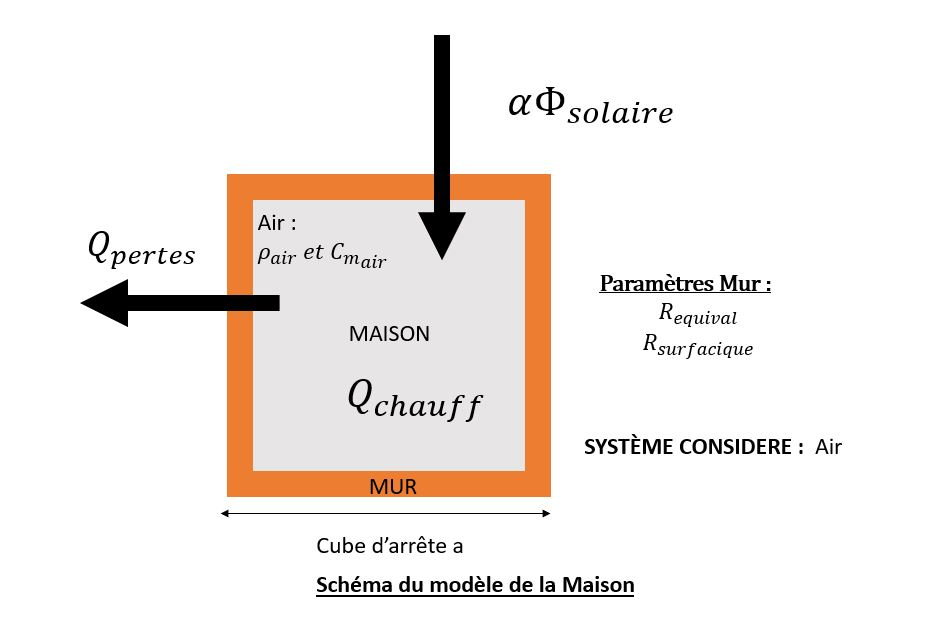
\includegraphics{modele.JPG}
\caption{Title}
\end{figure}

\hypertarget{moduxe8le-physique}{%
\paragraph{\texorpdfstring{\emph{\textbf{Modèle
Physique}}}{Modèle Physique}}\label{moduxe8le-physique}}

Si l'on considère une petite transformation pendant \(dt\). L'écriture
du premier principe à la maison \(\Sigma = { \ air \ à \ l'intérieur}\)
nous donne :
\[dU = C_{m}dT = Q_{chauffage} + Q_{Rayonnement} - Q_{Pertes}\] On
néglige \(Q_{anthropique}\).
\[C_{m}dT = w(t)dt + \alpha \Phi_sS_{ext}dt + \frac{T_{ext}-T}{R_{th}}dt\]
d'où:

\[\boxed{\frac{dT}{dt} + \frac{T}{R_{th}C_{m}} =\frac{1}{C_{m}}\Bigg[w(t) +\alpha \Phi_sS_{ext} +\frac{T_{ext}}{R_{th}}  \Bigg]}\]

\hypertarget{discruxe9tisation-du-probluxe8me}{%
\subsubsection{Discrétisation du
problème}\label{discruxe9tisation-du-probluxe8me}}

Dans le cadre général en notant \(T_i = T(\tau i)\), si \(\tau\) est
suffisament petit devant les durées de variation de \(w\), \(\Phi_s\) et
\(T\) on peut écrire :
\[\boxed{\Delta T= T_{i+1}-T_{i}=\frac{\tau}{C_{m}}[w(i\tau) +\alpha \Phi_s(\tau i )S_{ext} + \frac{T_{ext}(\tau i )-T_i}{R_{th}}]} \ \ - \ \ (E)\]

Dans le cadre des données fournies sur \(OASIS\). on a
\(\forall t, w(t) = 0\). D'où :
\[\Delta T= T_{i+1}-T_{i}=\frac{\tau}{C_{m}}[\alpha \Phi_s(\tau i )S_{ext} + \frac{T_{ext}(\tau i )-T_i}{R_{th}}]\]

Or si on fait l'hyphothèse d'une maison cubique de volume
\(V = S^{\frac{3}{2}}\). Or
\(C_m = C_{massique}\rho_{air}V = C_{massique}\rho_{air}S^{\frac{3}{2}}\).
D'où \(S = (\frac{C_m}{C_{massique}\rho_{air}})^{\frac{2}{3}}\)

Or on a \(C_{massique} = 1004 J.K^{-1}kg^{-1}\) et
\(\rho_{air} = 1 \ kg.m^{-3}\) - On remarque que on connait l'évolution
temporelle de la température de la maison pour \(W(t)=0\), ainsi que de
la température extéireure et l'ensoleillemnent associé - Les paramètres
de notre problème sont : - La longueur d'un côté \(a\) - La résistance
surfacique thermiques des murs, qui conditionne l'épaisseur des murs. -
La résistance thermique de l'ensemble de la maison. - La part \(\alpha\)
du flux solaire arrivant à chauffer l'air de la maison. - La capacité de
la maison \(C_m\)

\begin{itemize}
\item
  Cependant on décompte uniquement 3 variables signicatives que sont :
  \(R_{surf},\alpha\ et\ S_ext\). En effet :

  \begin{itemize}
  \tightlist
  \item
    \(R_{surf} = R_{th}.S_{ext}\) (On considère \(R_surf\) pour pouvoir
    juger rapidement de la faisabilité de l'épaisseur des murs
    modélisés, et donc de la cohérence du modèle)
  \item
    \(C_m = C_{massique}\rho_{air}a^3\)
  \item
    \(a = \sqrt{S_{ext}/5}\)
  \end{itemize}
\item
  On cherche donc les paramètres qui permettent d'approcher les
  différentes valeurs par une fonction respectant l'equation
  différentielle présentée plus haut.
\item
  \begin{quote}
  \textbf{Hypothèse} : On va supposer que la constante de discrétisation
  \(\tau\) est très petite devant la constante de temps du modèle
  \(\delta\). Par ailleurs \(w\) et \(\Phi_s et T_{ext}\) étant mesurée
  toutes les 30 minutes, on va les supposer constant sur cette durée.
  \end{quote}
\item
  Pour trouver les paramètres significatifs on effectue une regression
  en utilisant la méthode des moindres carrés. Cela revient à résoudre
  le problème d'optimisation suivant, en notant
  \(T,w,\Phi_s, T_{ext}, \Delta T\) les vecteurs de valeurs
  corespondantes aux temps d'observations : \[
  \min_{\alpha,S_{ext}, R_{surf} \in \mathbb{R}_+^3} {||{\frac{\tau}{C_{m}}[w +\alpha \Phi_sS_{ext} + \frac{(T_{ext}-T)S_{ext}}{R_{surf}}]-\Delta T}||}
  \]
\end{itemize}

    \begin{tcolorbox}[breakable, size=fbox, boxrule=1pt, pad at break*=1mm,colback=cellbackground, colframe=cellborder]
\prompt{In}{incolor}{1}{\boxspacing}
\begin{Verbatim}[commandchars=\\\{\}]
\PY{k+kn}{import} \PY{n+nn}{numpy} \PY{k}{as} \PY{n+nn}{np}
\PY{k+kn}{import} \PY{n+nn}{matplotlib}\PY{n+nn}{.}\PY{n+nn}{pyplot} \PY{k}{as} \PY{n+nn}{plt}
\PY{k+kn}{import} \PY{n+nn}{scipy}\PY{n+nn}{.}\PY{n+nn}{optimize} \PY{k}{as} \PY{n+nn}{optimize}
\end{Verbatim}
\end{tcolorbox}

    \begin{tcolorbox}[breakable, size=fbox, boxrule=1pt, pad at break*=1mm,colback=cellbackground, colframe=cellborder]
\prompt{In}{incolor}{2}{\boxspacing}
\begin{Verbatim}[commandchars=\\\{\}]
\PY{c+c1}{\PYZsh{} Extraction des données}
\PY{n}{data} \PY{o}{=} \PY{n}{np}\PY{o}{.}\PY{n}{loadtxt}\PY{p}{(}\PY{l+s+s1}{\PYZsq{}}\PY{l+s+s1}{donnees\PYZhy{}projet\PYZhy{}gr4.txt}\PY{l+s+s1}{\PYZsq{}}\PY{p}{)}
\PY{n}{heure} \PY{o}{=} \PY{n}{data}\PY{o}{.}\PY{n}{transpose}\PY{p}{(}\PY{p}{)}\PY{p}{[}\PY{l+m+mi}{0}\PY{p}{]}
\PY{n}{T\PYZus{}int} \PY{o}{=} \PY{n}{data}\PY{o}{.}\PY{n}{transpose}\PY{p}{(}\PY{p}{)}\PY{p}{[}\PY{l+m+mi}{1}\PY{p}{]}
\PY{n}{phi\PYZus{}sol} \PY{o}{=} \PY{n}{data}\PY{o}{.}\PY{n}{transpose}\PY{p}{(}\PY{p}{)}\PY{p}{[}\PY{l+m+mi}{2}\PY{p}{]}
\PY{n}{T\PYZus{}ext} \PY{o}{=} \PY{n}{data}\PY{o}{.}\PY{n}{transpose}\PY{p}{(}\PY{p}{)}\PY{p}{[}\PY{l+m+mi}{3}\PY{p}{]}
\PY{n}{plt}\PY{o}{.}\PY{n}{subplot}\PY{p}{(}\PY{p}{(}\PY{l+m+mi}{221}\PY{p}{)}\PY{p}{)}
\PY{n}{plt}\PY{o}{.}\PY{n}{plot}\PY{p}{(}\PY{n}{heure}\PY{p}{,}\PY{n}{T\PYZus{}int}\PY{p}{)}
\PY{n}{plt}\PY{o}{.}\PY{n}{title}\PY{p}{(}\PY{l+s+s1}{\PYZsq{}}\PY{l+s+s1}{températureint}\PY{l+s+s1}{\PYZsq{}}\PY{p}{)}
\PY{n}{plt}\PY{o}{.}\PY{n}{subplot}\PY{p}{(}\PY{p}{(}\PY{l+m+mi}{222}\PY{p}{)}\PY{p}{)}
\PY{n}{plt}\PY{o}{.}\PY{n}{plot}\PY{p}{(}\PY{n}{heure}\PY{p}{,}\PY{n}{phi\PYZus{}sol}\PY{p}{)}
\PY{n}{plt}\PY{o}{.}\PY{n}{title}\PY{p}{(}\PY{l+s+s1}{\PYZsq{}}\PY{l+s+s1}{flux solaire}\PY{l+s+s1}{\PYZsq{}}\PY{p}{)}
\PY{n}{plt}\PY{o}{.}\PY{n}{subplot}\PY{p}{(}\PY{l+m+mi}{223}\PY{p}{)}
\PY{n}{plt}\PY{o}{.}\PY{n}{plot}\PY{p}{(}\PY{n}{heure}\PY{p}{,}\PY{n}{T\PYZus{}ext}\PY{p}{)}
\PY{n}{plt}\PY{o}{.}\PY{n}{title}\PY{p}{(}\PY{l+s+s1}{\PYZsq{}}\PY{l+s+s1}{température \PYZus{}ext}\PY{l+s+s1}{\PYZsq{}}\PY{p}{)}
\PY{c+c1}{\PYZsh{}Création du vecteur des différences   }
\PY{n}{diff} \PY{o}{=} \PY{p}{[}\PY{p}{]}
\PY{k}{for} \PY{n}{i} \PY{o+ow}{in} \PY{n+nb}{range} \PY{p}{(}\PY{l+m+mi}{1}\PY{p}{,} \PY{n+nb}{len}\PY{p}{(}\PY{n}{T\PYZus{}int}\PY{p}{)}\PY{p}{)}\PY{p}{:}
    \PY{n}{diff}\PY{o}{.}\PY{n}{append}\PY{p}{(}\PY{n}{T\PYZus{}int}\PY{p}{[}\PY{n}{i}\PY{p}{]}\PY{o}{\PYZhy{}}\PY{n}{T\PYZus{}int}\PY{p}{[}\PY{n}{i}\PY{o}{\PYZhy{}}\PY{l+m+mi}{1}\PY{p}{]}\PY{p}{)}
\PY{n}{diff}  \PY{o}{=} \PY{n}{np}\PY{o}{.}\PY{n}{array}\PY{p}{(}\PY{n}{diff}\PY{p}{)}

\PY{n}{diff} \PY{o}{=} \PY{n}{diff}\PY{p}{[}\PY{l+m+mi}{1}\PY{p}{:}\PY{p}{]}\PY{c+c1}{\PYZsh{} On enlève les premières données pour qui faussent la régression}
\PY{n}{T\PYZus{}int} \PY{o}{=}\PY{n}{T\PYZus{}int}\PY{p}{[}\PY{l+m+mi}{2}\PY{p}{:}\PY{p}{]}\PY{c+c1}{\PYZsh{} On enlève les données inutilisables à cause de la taille inférieure du vecteur différence}
\PY{n}{phi\PYZus{}sol} \PY{o}{=} \PY{n}{phi\PYZus{}sol}\PY{p}{[}\PY{l+m+mi}{2}\PY{p}{:}\PY{p}{]}
\PY{n}{T\PYZus{}ext} \PY{o}{=} \PY{n}{T\PYZus{}ext}\PY{p}{[}\PY{l+m+mi}{2}\PY{p}{:}\PY{p}{]}
\PY{n}{heure} \PY{o}{=} \PY{n}{heure}\PY{p}{[}\PY{l+m+mi}{2}\PY{p}{:}\PY{p}{]}
\end{Verbatim}
\end{tcolorbox}

    \begin{center}
    \adjustimage{max size={0.9\linewidth}{0.9\paperheight}}{proj_opti_chesneaux_plessix_files/proj_opti_chesneaux_plessix_2_0.png}
    \end{center}
    { \hspace*{\fill} \\}
    
    \begin{tcolorbox}[breakable, size=fbox, boxrule=1pt, pad at break*=1mm,colback=cellbackground, colframe=cellborder]
\prompt{In}{incolor}{3}{\boxspacing}
\begin{Verbatim}[commandchars=\\\{\}]
\PY{c+c1}{\PYZsh{} Création de notre modèle Fonction qui trace l\PYZsq{}évolution de la température en fonction des paramètres}
\PY{c+c1}{\PYZsh{}  modélisation Méthode d\PYZsq{}euler}
\PY{c+c1}{\PYZsh{} a partir des paramètres et d\PYZsq{}une seule donnée de départ}

\PY{k}{def} \PY{n+nf}{mod1}\PY{p}{(}\PY{n}{T\PYZus{}0}\PY{p}{,}\PY{n}{T\PYZus{}ext}\PY{p}{,} \PY{n}{Phi\PYZus{}sol}\PY{p}{,}\PY{n}{tau}\PY{p}{,}\PY{n}{R}\PY{p}{,}\PY{n}{C}\PY{p}{,}\PY{n}{alpha}\PY{p}{,}\PY{n}{S\PYZus{}ext}\PY{p}{)}\PY{p}{:}
    \PY{n}{a} \PY{o}{=} \PY{p}{(}\PY{n}{S\PYZus{}ext}\PY{o}{/}\PY{l+m+mi}{5}\PY{p}{)}\PY{o}{*}\PY{o}{*}\PY{p}{(}\PY{l+m+mi}{1}\PY{o}{/}\PY{l+m+mi}{2}\PY{p}{)}
    \PY{n}{V} \PY{o}{=} \PY{n}{a}\PY{o}{*}\PY{o}{*}\PY{l+m+mi}{3} \PY{c+c1}{\PYZsh{} volume de la maison}
    \PY{n}{C} \PY{o}{=} \PY{l+m+mi}{1256}\PY{o}{*}\PY{n}{V} \PY{c+c1}{\PYZsh{} On considère la maison remplie uniquement d\PYZsq{}air}
    \PY{n}{model} \PY{o}{=} \PY{p}{[}\PY{n}{T\PYZus{}0}\PY{p}{]} \PY{c+c1}{\PYZsh{} On initialise à une température T\PYZus{}0 exacte}
    \PY{k}{for} \PY{n}{i} \PY{o+ow}{in} \PY{n+nb}{range}\PY{p}{(}\PY{l+m+mi}{1}\PY{p}{,}\PY{n+nb}{len}\PY{p}{(}\PY{n}{T\PYZus{}ext}\PY{p}{)}\PY{p}{)}\PY{p}{:}
        \PY{n}{diff} \PY{o}{=}\PY{p}{(}\PY{l+m+mi}{3600}\PY{o}{*}\PY{n}{tau}\PY{o}{/}\PY{n}{C}\PY{p}{)}\PY{o}{*}\PY{p}{(}\PY{p}{(}\PY{n}{alpha}\PY{o}{*}\PY{n}{Phi\PYZus{}sol}\PY{p}{[}\PY{n}{i}\PY{p}{]}\PY{p}{)}\PY{o}{*}\PY{n}{S\PYZus{}ext} \PY{o}{\PYZhy{}} \PY{p}{(}\PY{n}{model}\PY{p}{[}\PY{o}{\PYZhy{}}\PY{l+m+mi}{1}\PY{p}{]} \PY{o}{\PYZhy{}} \PY{n}{T\PYZus{}ext}\PY{p}{[}\PY{n}{i}\PY{p}{]}\PY{p}{)}\PY{o}{*}\PY{n}{S\PYZus{}ext}\PY{o}{/}\PY{n}{R}\PY{p}{)}
        \PY{n}{model}\PY{o}{.}\PY{n}{append}\PY{p}{(}\PY{n}{model}\PY{p}{[}\PY{o}{\PYZhy{}}\PY{l+m+mi}{1}\PY{p}{]} \PY{o}{+} \PY{n}{diff}\PY{p}{)}
    \PY{k}{return} \PY{n}{model}
\end{Verbatim}
\end{tcolorbox}

    \begin{tcolorbox}[breakable, size=fbox, boxrule=1pt, pad at break*=1mm,colback=cellbackground, colframe=cellborder]
\prompt{In}{incolor}{4}{\boxspacing}
\begin{Verbatim}[commandchars=\\\{\}]
\PY{c+c1}{\PYZsh{}modèle en supposant T\PYZus{}int connus et exactes}
\PY{c+c1}{\PYZsh{} S\PYZsq{}approche plus exactement de l\PYZsq{}approximation que fait l\PYZsq{}algortihme}
\PY{k}{def} \PY{n+nf}{mod2}\PY{p}{(}\PY{n}{T\PYZus{}0}\PY{p}{,}\PY{n}{T\PYZus{}ext}\PY{p}{,} \PY{n}{Phi\PYZus{}sol}\PY{p}{,}\PY{n}{tau}\PY{p}{,}\PY{n}{R}\PY{p}{,}\PY{n}{C}\PY{p}{,}\PY{n}{alpha}\PY{p}{,}\PY{n}{S\PYZus{}ext}\PY{p}{)}\PY{p}{:}
    \PY{n}{a} \PY{o}{=} \PY{p}{(}\PY{n}{S\PYZus{}ext}\PY{o}{/}\PY{l+m+mi}{5}\PY{p}{)}\PY{o}{*}\PY{o}{*}\PY{p}{(}\PY{l+m+mi}{1}\PY{o}{/}\PY{l+m+mi}{2}\PY{p}{)}
    \PY{n}{V} \PY{o}{=} \PY{n}{a}\PY{o}{*}\PY{o}{*}\PY{l+m+mi}{3} \PY{c+c1}{\PYZsh{} volume de la maison}
    \PY{n}{C} \PY{o}{=} \PY{l+m+mi}{1256}\PY{o}{*}\PY{n}{V} \PY{c+c1}{\PYZsh{} On considère la maison remplie uniquement d\PYZsq{}air}
    \PY{n}{model} \PY{o}{=} \PY{p}{[}\PY{n}{T\PYZus{}0}\PY{p}{]}
    \PY{k}{for} \PY{n}{i} \PY{o+ow}{in} \PY{n+nb}{range}\PY{p}{(}\PY{l+m+mi}{0}\PY{p}{,}\PY{n+nb}{len}\PY{p}{(}\PY{n}{T\PYZus{}ext}\PY{p}{)}\PY{o}{\PYZhy{}}\PY{l+m+mi}{1}\PY{p}{)}\PY{p}{:}
        \PY{n}{diff} \PY{o}{=}\PY{p}{(}\PY{l+m+mi}{3600}\PY{o}{*}\PY{n}{tau}\PY{o}{/}\PY{n}{C}\PY{p}{)}\PY{o}{*}\PY{p}{(}\PY{p}{(}\PY{n}{alpha}\PY{o}{*}\PY{n}{Phi\PYZus{}sol}\PY{p}{[}\PY{n}{i}\PY{p}{]}\PY{p}{)}\PY{o}{*}\PY{n}{S\PYZus{}ext} \PY{o}{\PYZhy{}} \PY{p}{(}\PY{n}{T\PYZus{}int} \PY{o}{\PYZhy{}} \PY{n}{T\PYZus{}ext}\PY{p}{[}\PY{n}{i}\PY{p}{]}\PY{p}{)}\PY{o}{*}\PY{n}{S\PYZus{}ext}\PY{o}{/}\PY{n}{R}\PY{p}{)}
        \PY{n}{model}\PY{o}{.}\PY{n}{append}\PY{p}{(}\PY{n}{T\PYZus{}int}\PY{p}{[}\PY{n}{i}\PY{p}{]} \PY{o}{+} \PY{n}{diff}\PY{p}{)}
    \PY{k}{return} \PY{n}{model}
\end{Verbatim}
\end{tcolorbox}

    \begin{tcolorbox}[breakable, size=fbox, boxrule=1pt, pad at break*=1mm,colback=cellbackground, colframe=cellborder]
\prompt{In}{incolor}{5}{\boxspacing}
\begin{Verbatim}[commandchars=\\\{\}]
\PY{c+c1}{\PYZsh{}Fonction de résidu}
\PY{c+c1}{\PYZsh{} X = [alpha, R\PYZus{}surf, S\PYZus{}ext]}

\PY{k}{def} \PY{n+nf}{f}\PY{p}{(}\PY{n}{x}\PY{p}{)}\PY{p}{:}
    \PY{n}{alpha} \PY{o}{=} \PY{n}{x}\PY{p}{[}\PY{l+m+mi}{0}\PY{p}{]}
    \PY{n}{R} \PY{o}{=} \PY{n}{x}\PY{p}{[}\PY{l+m+mi}{1}\PY{p}{]}
    \PY{n}{S\PYZus{}ext} \PY{o}{=} \PY{n}{x}\PY{p}{[}\PY{l+m+mi}{2}\PY{p}{]}
    \PY{n}{tau} \PY{o}{=} \PY{l+m+mf}{0.5}
    \PY{n}{a} \PY{o}{=} \PY{n}{np}\PY{o}{.}\PY{n}{sqrt}\PY{p}{(}\PY{n}{S\PYZus{}ext}\PY{o}{/}\PY{l+m+mi}{5}\PY{p}{)}
    \PY{n}{V} \PY{o}{=} \PY{n}{a}\PY{o}{*}\PY{o}{*}\PY{l+m+mi}{3} \PY{c+c1}{\PYZsh{} volume de la maison}
    \PY{n}{C} \PY{o}{=} \PY{l+m+mi}{1256}\PY{o}{*}\PY{n}{V} \PY{c+c1}{\PYZsh{} On considère la maison remplie uniquement d\PYZsq{}air}
    
    \PY{k}{return} \PY{p}{(}\PY{l+m+mi}{3600}\PY{o}{*}\PY{n}{tau}\PY{o}{/}\PY{n}{C}\PY{p}{)}\PY{o}{*}\PY{p}{(}\PY{p}{(}\PY{n}{alpha}\PY{o}{*}\PY{n}{phi\PYZus{}sol}\PY{o}{*}\PY{n}{S\PYZus{}ext}\PY{p}{)} \PY{o}{\PYZhy{}} \PY{p}{(}\PY{n}{T\PYZus{}int} \PY{o}{\PYZhy{}} \PY{n}{T\PYZus{}ext}\PY{p}{)}\PY{o}{*}\PY{n}{S\PYZus{}ext}\PY{o}{/}\PY{n}{R}\PY{p}{)}\PY{o}{\PYZhy{}}\PY{n}{diff}
\end{Verbatim}
\end{tcolorbox}

    \begin{tcolorbox}[breakable, size=fbox, boxrule=1pt, pad at break*=1mm,colback=cellbackground, colframe=cellborder]
\prompt{In}{incolor}{6}{\boxspacing}
\begin{Verbatim}[commandchars=\\\{\}]
\PY{c+c1}{\PYZsh{} Moindres carrés linéaires}
\PY{n+nb}{print}\PY{p}{(}\PY{n+nb}{len}\PY{p}{(}\PY{n}{diff}\PY{p}{)}\PY{p}{)}
\PY{n}{res} \PY{o}{=} \PY{n}{optimize}\PY{o}{.}\PY{n}{least\PYZus{}squares}\PY{p}{(}\PY{n}{f}\PY{p}{,}\PY{p}{[}\PY{l+m+mf}{0.1}\PY{p}{,}\PY{l+m+mi}{10}\PY{p}{,}\PY{l+m+mi}{100}\PY{p}{]}\PY{p}{,} \PY{n}{verbose}\PY{o}{=}\PY{l+m+mi}{1}\PY{p}{,} \PY{n}{method} \PY{o}{=}\PY{l+s+s1}{\PYZsq{}}\PY{l+s+s1}{trf}\PY{l+s+s1}{\PYZsq{}}\PY{p}{)}
\PY{n}{residual} \PY{o}{=} \PY{n}{res}\PY{o}{.}\PY{n}{fun}
\PY{n}{alpha}\PY{p}{,} \PY{n}{R}\PY{p}{,} \PY{n}{S\PYZus{}ext} \PY{o}{=} \PY{n}{res}\PY{o}{.}\PY{n}{x}
\PY{n}{a} \PY{o}{=} \PY{n}{np}\PY{o}{.}\PY{n}{sqrt}\PY{p}{(}\PY{n}{S\PYZus{}ext}\PY{o}{/}\PY{l+m+mi}{5}\PY{p}{)}
\PY{n}{V} \PY{o}{=} \PY{p}{(}\PY{n}{a}\PY{o}{*}\PY{o}{*}\PY{l+m+mi}{3}\PY{p}{)}  
\PY{n}{C} \PY{o}{=} \PY{l+m+mi}{1256}\PY{o}{*}\PY{n}{V}
\PY{c+c1}{\PYZsh{}\PYZsh{}\PYZsh{}\PYZsh{}\PYZsh{}\PYZsh{}\PYZsh{}\PYZsh{}\PYZsh{}\PYZsh{}\PYZsh{}\PYZsh{}\PYZsh{}\PYZsh{}\PYZsh{}\PYZsh{}\PYZsh{}\PYZsh{}\PYZsh{}\PYZsh{}\PYZsh{}\PYZsh{}\PYZsh{}\PYZsh{}\PYZsh{}\PYZsh{}\PYZsh{}\PYZsh{}\PYZsh{}\PYZsh{}\PYZsh{}\PYZsh{}\PYZsh{}\PYZsh{}\PYZsh{}\PYZsh{}\PYZsh{}\PYZsh{}\PYZsh{}}

\PY{n+nb}{print}\PY{p}{(}\PY{l+s+s1}{\PYZsq{}}\PY{l+s+s1}{===== }\PY{l+s+se}{\PYZbs{}n}\PY{l+s+s1}{\PYZsq{}}\PY{p}{)}
\PY{n+nb}{print}\PY{p}{(}\PY{l+s+s1}{\PYZsq{}}\PY{l+s+s1}{ MODELISATION DE LA MAISON }\PY{l+s+se}{\PYZbs{}n}\PY{l+s+s1}{ }\PY{l+s+s1}{\PYZsq{}}\PY{p}{)}
\PY{n+nb}{print}\PY{p}{(}\PY{l+s+s1}{\PYZsq{}}\PY{l+s+s1}{Murs de résistance équivalente}\PY{l+s+s1}{\PYZsq{}}\PY{p}{,} \PY{n}{R}\PY{o}{/}\PY{p}{(}\PY{n}{S\PYZus{}ext}\PY{p}{)}\PY{p}{,}\PY{l+s+s1}{\PYZsq{}}\PY{l+s+se}{\PYZbs{}n}\PY{l+s+s1}{\PYZsq{}}\PY{p}{)}
\PY{n+nb}{print}\PY{p}{(}\PY{l+s+s1}{\PYZsq{}}\PY{l+s+s1}{Surface extérieure}\PY{l+s+s1}{\PYZsq{}}\PY{p}{,} \PY{n}{S\PYZus{}ext}\PY{p}{,}\PY{l+s+s1}{\PYZsq{}}\PY{l+s+s1}{m² }\PY{l+s+se}{\PYZbs{}n}\PY{l+s+s1}{\PYZsq{}}\PY{p}{)}
\PY{n+nb}{print}\PY{p}{(}\PY{l+s+s1}{\PYZsq{}}\PY{l+s+s1}{Cube de côté a :}\PY{l+s+s1}{\PYZsq{}}\PY{p}{,} \PY{n}{np}\PY{o}{.}\PY{n}{sqrt}\PY{p}{(}\PY{n}{S\PYZus{}ext}\PY{o}{/}\PY{l+m+mi}{5}\PY{p}{)}\PY{p}{,} \PY{l+s+s1}{\PYZsq{}}\PY{l+s+s1}{m}\PY{l+s+s1}{\PYZsq{}}\PY{p}{,}\PY{l+s+s1}{\PYZsq{}}\PY{l+s+se}{\PYZbs{}n}\PY{l+s+s1}{\PYZsq{}}\PY{p}{)}
\PY{n+nb}{print}\PY{p}{(}\PY{l+s+s1}{\PYZsq{}}\PY{l+s+s1}{Mur de résistance surfacique}\PY{l+s+s1}{\PYZsq{}}\PY{p}{,}\PY{n}{R}\PY{p}{,}\PY{l+s+s1}{\PYZsq{}}\PY{l+s+s1}{m\PYZca{}2KW\PYZca{}\PYZhy{}1}\PY{l+s+se}{\PYZbs{}n}\PY{l+s+s1}{\PYZsq{}}\PY{p}{)} 
\PY{n+nb}{print}\PY{p}{(}\PY{l+s+s1}{\PYZsq{}}\PY{l+s+s1}{Pourcentage du flux solaire chauffant la maison}\PY{l+s+s1}{\PYZsq{}}\PY{p}{,} \PY{n}{alpha}\PY{p}{,}\PY{l+s+s1}{\PYZsq{}}\PY{l+s+se}{\PYZbs{}n}\PY{l+s+s1}{\PYZsq{}}\PY{p}{)}
\PY{n+nb}{print}\PY{p}{(}\PY{l+s+s1}{\PYZsq{}}\PY{l+s+s1}{Capacité thermique de la maison}\PY{l+s+s1}{\PYZsq{}}\PY{p}{,} \PY{n}{C}\PY{p}{,}\PY{l+s+s1}{\PYZsq{}}\PY{l+s+s1}{JK\PYZca{}\PYZhy{}1}\PY{l+s+se}{\PYZbs{}n}\PY{l+s+s1}{\PYZsq{}}\PY{p}{)}
\end{Verbatim}
\end{tcolorbox}

    \begin{Verbatim}[commandchars=\\\{\}]
142
`ftol` termination condition is satisfied.
Function evaluations 22, initial cost 2.6349e+03, final cost 1.8435e-01, first-
order optimality 1.98e-05.
=====

 MODELISATION DE LA MAISON

Murs de résistance équivalente 1.3505426600404253

Surface extérieure 301.23236459801774 m²

Cube de côté a : 7.7618601455838885 m

Mur de résistance surfacique 406.8271589744741 m\^{}2KW\^{}-1

Pourcentage du flux solaire chauffant la maison 0.0007411307540039446

Capacité thermique de la maison 587336.6195157372 JK\^{}-1

    \end{Verbatim}

    \begin{tcolorbox}[breakable, size=fbox, boxrule=1pt, pad at break*=1mm,colback=cellbackground, colframe=cellborder]
\prompt{In}{incolor}{7}{\boxspacing}
\begin{Verbatim}[commandchars=\\\{\}]
\PY{c+c1}{\PYZsh{} Vérification visuelle de la validité du modèle}
\PY{c+c1}{\PYZsh{} On suppose que la première valeur est exacte}
\PY{c+c1}{\PYZsh{} C\PYZsq{}est pour cela que l\PYZsq{}on a mis de coté la première valeur du jeu de données}
\PY{n}{model1} \PY{o}{=}  \PY{n}{mod1}\PY{p}{(}\PY{n}{T\PYZus{}int}\PY{p}{[}\PY{l+m+mi}{0}\PY{p}{]}\PY{p}{,}\PY{n}{T\PYZus{}ext}\PY{p}{,} \PY{n}{phi\PYZus{}sol}\PY{p}{,}\PY{l+m+mf}{0.5}\PY{p}{,}\PY{n}{R}\PY{p}{,}\PY{n}{C}\PY{p}{,}\PY{n}{alpha}\PY{p}{,}\PY{n}{S\PYZus{}ext}\PY{p}{)}
\PY{n}{plt}\PY{o}{.}\PY{n}{plot}\PY{p}{(}\PY{n}{heure}\PY{p}{,}\PY{n}{model1}\PY{p}{,} \PY{n}{label} \PY{o}{=} \PY{l+s+s2}{\PYZdq{}}\PY{l+s+s2}{meth1\PYZhy{}euler}\PY{l+s+s2}{\PYZdq{}}\PY{p}{)}
\PY{n}{plt}\PY{o}{.}\PY{n}{plot}\PY{p}{(}\PY{n}{heure}\PY{p}{,}\PY{n}{T\PYZus{}int}\PY{p}{,} \PY{n}{label} \PY{o}{=} \PY{l+s+s1}{\PYZsq{}}\PY{l+s+s1}{exp}\PY{l+s+s1}{\PYZsq{}}\PY{p}{)}
\PY{n}{plt}\PY{o}{.}\PY{n}{legend}\PY{p}{(}\PY{p}{)}
\PY{n}{plt}\PY{o}{.}\PY{n}{title}\PY{p}{(}\PY{l+s+s1}{\PYZsq{}}\PY{l+s+s1}{Valeurs exp et modélisation}\PY{l+s+s1}{\PYZsq{}}\PY{p}{)}
\end{Verbatim}
\end{tcolorbox}

            \begin{tcolorbox}[breakable, size=fbox, boxrule=.5pt, pad at break*=1mm, opacityfill=0]
\prompt{Out}{outcolor}{7}{\boxspacing}
\begin{Verbatim}[commandchars=\\\{\}]
Text(0.5, 1.0, 'Valeurs exp et modélisation')
\end{Verbatim}
\end{tcolorbox}
        
    \begin{center}
    \adjustimage{max size={0.9\linewidth}{0.9\paperheight}}{proj_opti_chesneaux_plessix_files/proj_opti_chesneaux_plessix_7_1.png}
    \end{center}
    { \hspace*{\fill} \\}
    
    \begin{quote}
On a ici choisit la méthode dite \texttt{trf}, car celle-ci parcourt
tout l'espace pour déterminer la solution optimale, cela permet dans le
cas où il y'a de nombreux minimas locaux, de chercher l'extremum global
dans tout l'espace. ( c'est le cas ici)
\end{quote}

On voit après calcul que le produit \(RC_m\) est très grand devant
\(\tau\). Donc la discrétisation réalisée est acceptable. Cependant la
discrétisation des températures et du flux solaire est quand à elle plus
discutable. Essentiellement pour le flux solaire qui a des variations
très brusques et importantes. Ce qui peut entrainer une surévaluation
des flux entrants considérés. On aurait pu faire une approximation à la
méthode des trapèzes des quantités considérées.

    \hypertarget{conclusion}{%
\paragraph{Conclusion}\label{conclusion}}

On peut voir visuellement que ce modèle implémenté avec paramètres suit
assez bien la courbe de l'évolution de la température. \textbf{Le modèle
en lui même est donc acceptable.}

Cependant pour ce qui est de la \textbf{cohérence des paramètres}. On
remarque que la taille de la maison est cohérente, et correspond à à peu
près une maison entre 60 et 100 m2. Le taux d'utilisation du rayonnement
solaire est plutôt faible, mais ce qui n'est pas extrèmement alarmant,
lorsqu'on sait que l'on a pu considérer uen grande partie du rayonnement
incident sur une surface opaque, la majeur partie du rayonnement est
donc réemis par la maison. Le point préoccupant reste cependant la
valeur de la résistance thermique surfacique de la maison qui est
beaucoup trop élevée (facteur 100 ) il faut savoir que on recommande
généralement d'équiper sa maison avec des murs de résistance de l'ordre
4/5.

    \hypertarget{limites}{%
\paragraph{Limites}\label{limites}}

Un point à vérifier serait la qualité des mesures et les conditions de
l'expérience qui ne sont pas exactement connues, on part ici du postulat
qu'elle sont parfaites. Par exemple, lorsqu'on regarde le décrochage de
température à 65h, on remarque que les conditions sont moins favorable
que au pic de 10h. En effet la température extérieure est plus
importante à 65h et donc la pertes de chaleur devrait être au moins plus
petites. Or c'est l'inverse, cela pourrait être du à une fenêtre une
porte ouverte. Ou alors une pluie qui refroidit les murs et qui donc
augmente les pertes et baisse l'apport solaire. Cela nous permettrait de
faire intervenir des incertitudes qui permettraient

    \hypertarget{autre-approche}{%
\paragraph{Autre approche}\label{autre-approche}}

On a ici fait le choix de trouver les paramètres qui permettent de
valider le plus possible le modèle on aurait aussi pu déterminer les
paramètres qui permettent d'approcher le plus possible la température.
Cela revient à proposer de résoudre le problème suivant : \[
\min_{\alpha, R_{th}, R_{surf} \in \mathbb{R}_+^3} {||T_{expérimental}-T||}
\] sachant que \(T\) suit la dynamique physique présentée plus haut,
dépendant de \(\alpha, R_{th} \ et \ R_{surf}\).

    \begin{tcolorbox}[breakable, size=fbox, boxrule=1pt, pad at break*=1mm,colback=cellbackground, colframe=cellborder]
\prompt{In}{incolor}{8}{\boxspacing}
\begin{Verbatim}[commandchars=\\\{\}]
\PY{c+c1}{\PYZsh{} Extraction des données}
\PY{n}{data} \PY{o}{=} \PY{n}{np}\PY{o}{.}\PY{n}{loadtxt}\PY{p}{(}\PY{l+s+s1}{\PYZsq{}}\PY{l+s+s1}{donnees\PYZhy{}projet\PYZhy{}gr4.txt}\PY{l+s+s1}{\PYZsq{}}\PY{p}{)}
\PY{n}{data} \PY{o}{=} \PY{n}{data}\PY{p}{[}\PY{l+m+mi}{3}\PY{p}{:}\PY{p}{]} \PY{c+c1}{\PYZsh{}même simplification que plus haut}
\PY{n}{heure} \PY{o}{=} \PY{n}{data}\PY{o}{.}\PY{n}{transpose}\PY{p}{(}\PY{p}{)}\PY{p}{[}\PY{l+m+mi}{0}\PY{p}{]}
\PY{n}{T\PYZus{}int} \PY{o}{=} \PY{n}{data}\PY{o}{.}\PY{n}{transpose}\PY{p}{(}\PY{p}{)}\PY{p}{[}\PY{l+m+mi}{1}\PY{p}{]}
\PY{n}{phi\PYZus{}sol} \PY{o}{=} \PY{n}{data}\PY{o}{.}\PY{n}{transpose}\PY{p}{(}\PY{p}{)}\PY{p}{[}\PY{l+m+mi}{2}\PY{p}{]}
\PY{n}{T\PYZus{}ext} \PY{o}{=} \PY{n}{data}\PY{o}{.}\PY{n}{transpose}\PY{p}{(}\PY{p}{)}\PY{p}{[}\PY{l+m+mi}{3}\PY{p}{]}
\PY{n}{plt}\PY{o}{.}\PY{n}{subplot}\PY{p}{(}\PY{p}{(}\PY{l+m+mi}{221}\PY{p}{)}\PY{p}{)}
\PY{n}{plt}\PY{o}{.}\PY{n}{plot}\PY{p}{(}\PY{n}{heure}\PY{p}{,}\PY{n}{T\PYZus{}int}\PY{p}{)}
\PY{n}{plt}\PY{o}{.}\PY{n}{title}\PY{p}{(}\PY{l+s+s1}{\PYZsq{}}\PY{l+s+s1}{températureint}\PY{l+s+s1}{\PYZsq{}}\PY{p}{)}
\PY{n}{plt}\PY{o}{.}\PY{n}{subplot}\PY{p}{(}\PY{p}{(}\PY{l+m+mi}{222}\PY{p}{)}\PY{p}{)}
\PY{n}{plt}\PY{o}{.}\PY{n}{plot}\PY{p}{(}\PY{n}{heure}\PY{p}{,}\PY{n}{phi\PYZus{}sol}\PY{p}{)}
\PY{n}{plt}\PY{o}{.}\PY{n}{title}\PY{p}{(}\PY{l+s+s1}{\PYZsq{}}\PY{l+s+s1}{flux solaire}\PY{l+s+s1}{\PYZsq{}}\PY{p}{)}
\PY{n}{plt}\PY{o}{.}\PY{n}{subplot}\PY{p}{(}\PY{l+m+mi}{223}\PY{p}{)}
\PY{n}{plt}\PY{o}{.}\PY{n}{plot}\PY{p}{(}\PY{n}{heure}\PY{p}{,}\PY{n}{T\PYZus{}ext}\PY{p}{)}
\PY{n}{plt}\PY{o}{.}\PY{n}{title}\PY{p}{(}\PY{l+s+s1}{\PYZsq{}}\PY{l+s+s1}{température \PYZus{}ext}\PY{l+s+s1}{\PYZsq{}}\PY{p}{)}
\end{Verbatim}
\end{tcolorbox}

            \begin{tcolorbox}[breakable, size=fbox, boxrule=.5pt, pad at break*=1mm, opacityfill=0]
\prompt{Out}{outcolor}{8}{\boxspacing}
\begin{Verbatim}[commandchars=\\\{\}]
Text(0.5, 1.0, 'température \_ext')
\end{Verbatim}
\end{tcolorbox}
        
    \begin{center}
    \adjustimage{max size={0.9\linewidth}{0.9\paperheight}}{proj_opti_chesneaux_plessix_files/proj_opti_chesneaux_plessix_12_1.png}
    \end{center}
    { \hspace*{\fill} \\}
    
    \begin{tcolorbox}[breakable, size=fbox, boxrule=1pt, pad at break*=1mm,colback=cellbackground, colframe=cellborder]
\prompt{In}{incolor}{9}{\boxspacing}
\begin{Verbatim}[commandchars=\\\{\}]
\PY{k}{def} \PY{n+nf}{least\PYZus{}square}\PY{p}{(}\PY{n}{T\PYZus{}0}\PY{p}{,}\PY{n}{T\PYZus{}int}\PY{p}{,} \PY{n}{T\PYZus{}ext}\PY{p}{,} \PY{n}{phi\PYZus{}sol}\PY{p}{)}\PY{p}{:}
    \PY{k}{def} \PY{n+nf}{f}\PY{p}{(}\PY{n}{X}\PY{p}{)}\PY{p}{:}
        \PY{k}{return} \PY{p}{(}\PY{n}{T\PYZus{}int}\PY{o}{\PYZhy{}}\PY{n}{mod1}\PY{p}{(}\PY{n}{T\PYZus{}0}\PY{p}{,}\PY{n}{T\PYZus{}ext}\PY{p}{,}\PY{n}{phi\PYZus{}sol}\PY{p}{,}\PY{l+m+mf}{0.5}\PY{p}{,}\PY{n}{X}\PY{p}{[}\PY{l+m+mi}{0}\PY{p}{]}\PY{p}{,}\PY{l+m+mi}{0}\PY{p}{,}\PY{n}{X}\PY{p}{[}\PY{l+m+mi}{1}\PY{p}{]}\PY{p}{,}\PY{n}{X}\PY{p}{[}\PY{l+m+mi}{2}\PY{p}{]}\PY{p}{)}\PY{p}{)}
    \PY{n}{res} \PY{o}{=} \PY{n}{optimize}\PY{o}{.}\PY{n}{least\PYZus{}squares}\PY{p}{(}\PY{n}{f}\PY{p}{,}\PY{p}{[}\PY{l+m+mi}{400}\PY{p}{,}\PY{l+m+mf}{0.001}\PY{p}{,}\PY{l+m+mi}{400}\PY{p}{]}\PY{p}{,} \PY{n}{verbose} \PY{o}{=} \PY{l+m+mi}{1}\PY{p}{,} \PY{n}{method} \PY{o}{=} \PY{l+s+s1}{\PYZsq{}}\PY{l+s+s1}{lm}\PY{l+s+s1}{\PYZsq{}}\PY{p}{)}
    \PY{k}{return} \PY{n}{res}\PY{o}{.}\PY{n}{x}\PY{p}{,} \PY{n}{res}\PY{o}{.}\PY{n}{cost}
\PY{c+c1}{\PYZsh{} La méthode est moins stable}
\PY{n}{res}\PY{p}{,}\PY{n}{cost} \PY{o}{=} \PY{n}{least\PYZus{}square}\PY{p}{(}\PY{n}{T\PYZus{}int}\PY{p}{[}\PY{l+m+mi}{0}\PY{p}{]}\PY{p}{,}\PY{n}{T\PYZus{}int}\PY{p}{,}\PY{n}{T\PYZus{}ext}\PY{p}{,}\PY{n}{phi\PYZus{}sol}\PY{p}{)}
\PY{n}{R}\PY{p}{,}\PY{n}{alpha}\PY{p}{,}\PY{n}{S\PYZus{}ext} \PY{o}{=} \PY{n}{res}
\PY{n+nb}{print}\PY{p}{(}\PY{l+s+s1}{\PYZsq{}}\PY{l+s+s1}{cost}\PY{l+s+s1}{\PYZsq{}}\PY{p}{,}\PY{n}{cost}\PY{p}{)}
\PY{n}{a} \PY{o}{=} \PY{n}{np}\PY{o}{.}\PY{n}{sqrt}\PY{p}{(}\PY{n}{S\PYZus{}ext}\PY{o}{/}\PY{l+m+mi}{5}\PY{p}{)}
\PY{n}{V} \PY{o}{=} \PY{n}{a}\PY{o}{*}\PY{o}{*}\PY{l+m+mi}{3}
\PY{n}{C} \PY{o}{=} \PY{l+m+mi}{1256}\PY{o}{*}\PY{n}{V}
\PY{c+c1}{\PYZsh{}}
\end{Verbatim}
\end{tcolorbox}

    \begin{Verbatim}[commandchars=\\\{\}]
`ftol` termination condition is satisfied.
Function evaluations 28, initial cost 1.0071e+01, final cost 9.8959e-01, first-
order optimality 7.92e-02.
cost 0.9895874898198811
    \end{Verbatim}

    \begin{tcolorbox}[breakable, size=fbox, boxrule=1pt, pad at break*=1mm,colback=cellbackground, colframe=cellborder]
\prompt{In}{incolor}{10}{\boxspacing}
\begin{Verbatim}[commandchars=\\\{\}]
\PY{n+nb}{print}\PY{p}{(}\PY{l+s+s1}{\PYZsq{}}\PY{l+s+s1}{===== }\PY{l+s+se}{\PYZbs{}n}\PY{l+s+s1}{\PYZsq{}}\PY{p}{)}
\PY{n+nb}{print}\PY{p}{(}\PY{l+s+s1}{\PYZsq{}}\PY{l+s+s1}{ MODELISATION DE LA MAISON }\PY{l+s+se}{\PYZbs{}n}\PY{l+s+s1}{ }\PY{l+s+s1}{\PYZsq{}}\PY{p}{)}
\PY{n+nb}{print}\PY{p}{(}\PY{l+s+s1}{\PYZsq{}}\PY{l+s+s1}{Murs de résistance équivalente}\PY{l+s+s1}{\PYZsq{}}\PY{p}{,} \PY{n}{R}\PY{o}{/}\PY{p}{(}\PY{n}{S\PYZus{}ext}\PY{p}{)}\PY{p}{,}\PY{l+s+s1}{\PYZsq{}}\PY{l+s+se}{\PYZbs{}n}\PY{l+s+s1}{\PYZsq{}}\PY{p}{)}
\PY{n+nb}{print}\PY{p}{(}\PY{l+s+s1}{\PYZsq{}}\PY{l+s+s1}{Surface extérieure}\PY{l+s+s1}{\PYZsq{}}\PY{p}{,} \PY{n}{S\PYZus{}ext}\PY{p}{,}\PY{l+s+s1}{\PYZsq{}}\PY{l+s+se}{\PYZbs{}n}\PY{l+s+s1}{\PYZsq{}}\PY{p}{)}
\PY{n+nb}{print}\PY{p}{(}\PY{l+s+s1}{\PYZsq{}}\PY{l+s+s1}{Cube de côté a :}\PY{l+s+s1}{\PYZsq{}}\PY{p}{,} \PY{n}{np}\PY{o}{.}\PY{n}{sqrt}\PY{p}{(}\PY{n}{S\PYZus{}ext}\PY{o}{/}\PY{l+m+mi}{5}\PY{p}{)}\PY{p}{,} \PY{l+s+s1}{\PYZsq{}}\PY{l+s+s1}{m}\PY{l+s+s1}{\PYZsq{}}\PY{p}{,}\PY{l+s+s1}{\PYZsq{}}\PY{l+s+se}{\PYZbs{}n}\PY{l+s+s1}{\PYZsq{}}\PY{p}{)}
\PY{n+nb}{print}\PY{p}{(}\PY{l+s+s1}{\PYZsq{}}\PY{l+s+s1}{Mur de résistance surfacique}\PY{l+s+s1}{\PYZsq{}}\PY{p}{,}\PY{n}{R}\PY{p}{,}\PY{l+s+s1}{\PYZsq{}}\PY{l+s+s1}{m\PYZca{}2KW\PYZca{}\PYZhy{}1}\PY{l+s+se}{\PYZbs{}n}\PY{l+s+s1}{\PYZsq{}}\PY{p}{)} 
\PY{n+nb}{print}\PY{p}{(}\PY{l+s+s1}{\PYZsq{}}\PY{l+s+s1}{Pourcentage du flux solaire chauffant la maison}\PY{l+s+s1}{\PYZsq{}}\PY{p}{,} \PY{n}{alpha}\PY{p}{,}\PY{l+s+s1}{\PYZsq{}}\PY{l+s+se}{\PYZbs{}n}\PY{l+s+s1}{\PYZsq{}}\PY{p}{)}
\PY{n+nb}{print}\PY{p}{(}\PY{l+s+s1}{\PYZsq{}}\PY{l+s+s1}{Capacité thermique de la maison}\PY{l+s+s1}{\PYZsq{}}\PY{p}{,} \PY{n}{C}\PY{p}{,}\PY{l+s+s1}{\PYZsq{}}\PY{l+s+s1}{JK\PYZca{}\PYZhy{}1}\PY{l+s+se}{\PYZbs{}n}\PY{l+s+s1}{\PYZsq{}}\PY{p}{)}
\end{Verbatim}
\end{tcolorbox}

    \begin{Verbatim}[commandchars=\\\{\}]
=====

 MODELISATION DE LA MAISON

Murs de résistance équivalente 0.7608983572190919

Surface extérieure 478.3693072702498

Cube de côté a : 9.781301623712968 m

Mur de résistance surfacique 363.9904200459681 m\^{}2KW\^{}-1

Pourcentage du flux solaire chauffant la maison 0.0007668921947591089

Capacité thermique de la maison 1175383.5098625598 JK\^{}-1

    \end{Verbatim}

    \begin{tcolorbox}[breakable, size=fbox, boxrule=1pt, pad at break*=1mm,colback=cellbackground, colframe=cellborder]
\prompt{In}{incolor}{11}{\boxspacing}
\begin{Verbatim}[commandchars=\\\{\}]
\PY{n}{model2} \PY{o}{=} \PY{n}{mod1}\PY{p}{(}\PY{n}{T\PYZus{}int}\PY{p}{[}\PY{l+m+mi}{0}\PY{p}{]}\PY{p}{,}\PY{n}{T\PYZus{}ext}\PY{p}{,} \PY{n}{phi\PYZus{}sol}\PY{p}{,}\PY{l+m+mf}{0.5}\PY{p}{,}\PY{n}{R}\PY{p}{,}\PY{n}{C}\PY{p}{,}\PY{n}{alpha}\PY{p}{,}\PY{n}{S\PYZus{}ext}\PY{p}{)}
\PY{n}{fig}\PY{p}{,} \PY{n}{ax1} \PY{o}{=} \PY{n}{plt}\PY{o}{.}\PY{n}{subplots}\PY{p}{(}\PY{p}{)}

\PY{n}{ax1}\PY{o}{.}\PY{n}{plot}\PY{p}{(}\PY{n}{heure}\PY{p}{,}\PY{n}{T\PYZus{}int}\PY{p}{,} \PY{n}{label} \PY{o}{=} \PY{l+s+s2}{\PYZdq{}}\PY{l+s+s2}{Val Expérimentale}\PY{l+s+s2}{\PYZdq{}}\PY{p}{)}
\PY{n}{ax1}\PY{o}{.}\PY{n}{plot}\PY{p}{(}\PY{n}{heure}\PY{p}{,}\PY{n}{model2}\PY{p}{,}\PY{n}{label} \PY{o}{=} \PY{l+s+s1}{\PYZsq{}}\PY{l+s+s1}{Modèle}\PY{l+s+s1}{\PYZsq{}}\PY{p}{)}

\PY{n}{ax1}\PY{o}{.}\PY{n}{legend}\PY{p}{(}\PY{p}{)}
\PY{n}{plt}\PY{o}{.}\PY{n}{title}\PY{p}{(}\PY{l+s+s1}{\PYZsq{}}\PY{l+s+s1}{Visualisation du modèle}\PY{l+s+s1}{\PYZsq{}}\PY{p}{)}
\PY{n}{plt}\PY{o}{.}\PY{n}{show}\PY{p}{(}\PY{p}{)}
\end{Verbatim}
\end{tcolorbox}

    \begin{center}
    \adjustimage{max size={0.9\linewidth}{0.9\paperheight}}{proj_opti_chesneaux_plessix_files/proj_opti_chesneaux_plessix_15_0.png}
    \end{center}
    { \hspace*{\fill} \\}
    
    \begin{tcolorbox}[breakable, size=fbox, boxrule=1pt, pad at break*=1mm,colback=cellbackground, colframe=cellborder]
\prompt{In}{incolor}{12}{\boxspacing}
\begin{Verbatim}[commandchars=\\\{\}]
\PY{c+c1}{\PYZsh{} Comparaison }
\PY{n}{plt}\PY{o}{.}\PY{n}{plot}\PY{p}{(}\PY{n}{heure}\PY{p}{,} \PY{n}{model1}\PY{p}{[}\PY{l+m+mi}{1}\PY{p}{:}\PY{p}{]}\PY{p}{,} \PY{n}{label} \PY{o}{=} \PY{l+s+s1}{\PYZsq{}}\PY{l+s+s1}{method1}\PY{l+s+s1}{\PYZsq{}}\PY{p}{)}
\PY{n}{plt}\PY{o}{.}\PY{n}{plot}\PY{p}{(}\PY{n}{heure}\PY{p}{,} \PY{n}{model2}\PY{p}{,} \PY{n}{label} \PY{o}{=} \PY{l+s+s1}{\PYZsq{}}\PY{l+s+s1}{method2}\PY{l+s+s1}{\PYZsq{}}\PY{p}{)}
\PY{n}{plt}\PY{o}{.}\PY{n}{plot}\PY{p}{(}\PY{n}{heure}\PY{p}{,} \PY{n}{T\PYZus{}int}\PY{p}{,} \PY{n}{label} \PY{o}{=} \PY{l+s+s1}{\PYZsq{}}\PY{l+s+s1}{exp}\PY{l+s+s1}{\PYZsq{}}\PY{p}{)}
\PY{n}{plt}\PY{o}{.}\PY{n}{legend}\PY{p}{(}\PY{p}{)}
\PY{n}{plt}\PY{o}{.}\PY{n}{title}\PY{p}{(}\PY{l+s+s1}{\PYZsq{}}\PY{l+s+s1}{Comparaison des deux méthodes}\PY{l+s+s1}{\PYZsq{}}\PY{p}{)}
\PY{n}{plt}\PY{o}{.}\PY{n}{show}\PY{p}{(}\PY{p}{)}
\PY{n+nb}{print}\PY{p}{(}\PY{l+s+s1}{\PYZsq{}}\PY{l+s+s1}{norme met2}\PY{l+s+s1}{\PYZsq{}}\PY{p}{,}\PY{n}{np}\PY{o}{.}\PY{n}{linalg}\PY{o}{.}\PY{n}{norm}\PY{p}{(}\PY{n}{T\PYZus{}int} \PY{o}{\PYZhy{}} \PY{n}{model2}\PY{p}{)}\PY{p}{)}
\PY{n}{plt}\PY{o}{.}\PY{n}{plot}\PY{p}{(}\PY{n}{heure}\PY{p}{,} \PY{n+nb}{abs}\PY{p}{(}\PY{n}{T\PYZus{}int} \PY{o}{\PYZhy{}} \PY{n}{model1}\PY{p}{[}\PY{l+m+mi}{1}\PY{p}{:}\PY{p}{]}\PY{p}{)}\PY{p}{,} \PY{n}{label} \PY{o}{=} \PY{l+s+s1}{\PYZsq{}}\PY{l+s+s1}{method1}\PY{l+s+s1}{\PYZsq{}}\PY{p}{)}
\PY{n}{plt}\PY{o}{.}\PY{n}{plot}\PY{p}{(}\PY{n}{heure}\PY{p}{,} \PY{n+nb}{abs}\PY{p}{(}\PY{n}{T\PYZus{}int}\PY{o}{\PYZhy{}}\PY{n}{model2}\PY{p}{)}\PY{p}{,} \PY{n}{label} \PY{o}{=} \PY{l+s+s2}{\PYZdq{}}\PY{l+s+s2}{method2}\PY{l+s+s2}{\PYZdq{}}\PY{p}{)}
\PY{n}{plt}\PY{o}{.}\PY{n}{legend}\PY{p}{(}\PY{p}{)}
\PY{n}{plt}\PY{o}{.}\PY{n}{title}\PY{p}{(}\PY{l+s+s1}{\PYZsq{}}\PY{l+s+s1}{comparaison des résidus}\PY{l+s+s1}{\PYZsq{}}\PY{p}{)}
\PY{n}{plt}\PY{o}{.}\PY{n}{show}\PY{p}{(}\PY{p}{)}
\PY{n+nb}{print}\PY{p}{(}\PY{l+s+s1}{\PYZsq{}}\PY{l+s+s1}{norme met1}\PY{l+s+s1}{\PYZsq{}}\PY{p}{,}\PY{n}{np}\PY{o}{.}\PY{n}{linalg}\PY{o}{.}\PY{n}{norm}\PY{p}{(}\PY{n}{T\PYZus{}int} \PY{o}{\PYZhy{}} \PY{n}{model1}\PY{p}{[}\PY{l+m+mi}{1}\PY{p}{:}\PY{p}{]}\PY{p}{)}\PY{p}{)}
\end{Verbatim}
\end{tcolorbox}

    \begin{center}
    \adjustimage{max size={0.9\linewidth}{0.9\paperheight}}{proj_opti_chesneaux_plessix_files/proj_opti_chesneaux_plessix_16_0.png}
    \end{center}
    { \hspace*{\fill} \\}
    
    \begin{Verbatim}[commandchars=\\\{\}]
norme met2 1.4068315391829123
    \end{Verbatim}

    \begin{center}
    \adjustimage{max size={0.9\linewidth}{0.9\paperheight}}{proj_opti_chesneaux_plessix_files/proj_opti_chesneaux_plessix_16_2.png}
    \end{center}
    { \hspace*{\fill} \\}
    
    \begin{Verbatim}[commandchars=\\\{\}]
norme met1 1.4863105780228225
    \end{Verbatim}

    On remarque que du \textbf{point de vue de l'approximation de la
température} la seconde méthode est meilleure car plus proche de la
température réelle. Cependant du \textbf{point de vue de l'approximation
du modèle} cette méthode est plus \textbf{faibl}e en effet à terme la
fonction de coût serait de 0.6 avec ces paramètres quand elle est de 0.1
avec les paramètres trouvés avec la première méthode (\textbf{Cela
présuppose que l'on considère toute les valeurs de températures
exactes}). Cependant elle est soumis à une incertitude du fait de
l'erreur accumulée par méthode de Euler on lui préferera donc la
première méthode. Les ordres de grandeurs des paramètres restent tout de
même les mêmes. L'interet de la méthode 2 est que l'on converge en moins
d'itérations que avec la méthode 1.

On retrouve toujours les mêmes problèmes de paramètres.

    \hypertarget{probluxe8me-doptimisation}{%
\subsubsection{Problème
d'optimisation}\label{probluxe8me-doptimisation}}

On cherche maintenant à optimiser la consommation de façon à diminuer la
facture d'électricité. Les contraintes physiques obligent \textbf{T à
respecter la loi} que nous avons défini plus tôt (en \(E\)). De plus le
radiateur consomme de l'electricité avec \textbf{une charge positive et
inférieure à une charge maximale}. Enfin la condition de confort des
usagers, est d'assurer une \textbf{température comprise entre une borne
inférieure et supérieure} à toute heure de la journée.

Le problème d'optimisation est donc après discrétisation :
\[ {min}_{(w_i), i\in {1,..,N}} P(x)= \sum_{i=1}^N{p}_i^{p/c}w_i\tau \]
s.t. \[ 0 \leq w_i \leq w_{max} -(1-2) \]
\[  20 ° C \leq Ti \leq 21°C - (3-4)\]
\[ T  \ vérifie \ (E) \ sous \ les \ paramètres \ déterminées\ au \  I.\ -(5)\]


    % Add a bibliography block to the postdoc
    
    
    
\end{document}
